\subsection{Margók}

%42
\begin{frame}
  A margók mindig átlátszók, csak a szélességük állítható:
  \begin{itemize}
    \item 1-4 érték megadásával, pl.\\
    \texttt{margin: 10px 20px 30px 40px;}\\
    (Fent, jobbra, lent, balra; további esetek mint \texttt{border-style}-nál.)
    \item Oldalakra vonatkozó tulajdonságokkal:\\
      \texttt{margin-*}, ahol \texttt{*} helyén állhat 
      \texttt{top}, \texttt{right}, \texttt{bottom}, \texttt{left}.
  \end{itemize}
\end{frame}

%43
\begin{frame}
  A margó szélessége lehet:
  \begin{itemize}
    \item \texttt{auto}: a tartalom által fel nem használt helyet felosztja egyenlően a bal és jobb oldal közt $\to$ középre igazít
    \item \texttt{inherit}: a befoglaló, szülő elem beállításait örökli
    \item CSS mértékegységgel (pl. \texttt{px}, \texttt{cm}) adott
    \item \texttt{\%}: a szülő elem méretének százaléka
  \end{itemize}
  \vfill
  Negatív értékek is használhatók.
\end{frame}

%_
\begin{frame}
  Az ablak keskenyebb, mint az elem \emph{rögzített} szélessége? $\to$ gördítősáv. \emph{Maximális} szélesség $\to$ csökkenthető. Középre igazítás: \texttt{margin: auto}-val.
  \begin{columns}[c]
    \column{0.55\textwidth}
      \begin{exampleblock}{\textattachfile{kozepre.html}{kozepre.html}}
        \fontsize{7}{8} \selectfont
        \lstinputlisting[style=HTML,linerange={7-7},numbers=left,firstnumber=7]{kozepre.html}
        \lstinputlisting[style=HTML,linerange={12-15},numbers=left,firstnumber=12]{kozepre.html}
        \lstinputlisting[style=HTML,linerange={19-21},numbers=left,firstnumber=19]{kozepre.html}
      \end{exampleblock}
    \column{0.25\textwidth}
      \includegraphics[width=\textwidth]{kozepre1.png}
    \column{0.15\textwidth}
      \includegraphics[width=\textwidth]{kozepre2.png}
  \end{columns}
\end{frame}

%44
\begin{frame}
  A blokkok felső és alsó margói időnként összeolvadnak, és a kettő közül csak a nagyobb marad meg:
  \begin{itemize}
    \item szülő szomszédos gyerekei között (szélső gyerekek 
    margói túlnyúlnak a szülőn)
    \item ha nincs olyan megjeleníthető szegély, kitöltés, stb., 
    ami elválasztaná a szülő és valamely gyerekének alsó/felső margóját
    \item üres blokkok alsó és felső margóját is összevonják
  \end{itemize}
  \vfill
  \hiv{\href{https://developer.mozilla.org/en-US/docs/Web/CSS/CSS\_Box\_Model/Mastering\_margin\_collapsing}{További részletek}}
\end{frame}

%45
\begin{frame}
  \begin{columns}[T]
    \column{0.45\textwidth}
      \begin{exampleblock}{\textattachfile{margok.html}{margok.html}}
        \scriptsize
        \lstinputlisting[style=HTML,linerange={7-16},numbers=left,firstnumber=7]{margok.html}
      \end{exampleblock}
    \column{0.45\textwidth}
      \begin{exampleblock}{\vspace*{-3ex}}
        \scriptsize
        \lstinputlisting[style=HTML,linerange={20-34},numbers=left,firstnumber=20]{margok.html}
      \end{exampleblock}
  \end{columns} 
\end{frame}

%46
\begin{frame}
  \begin{center}
    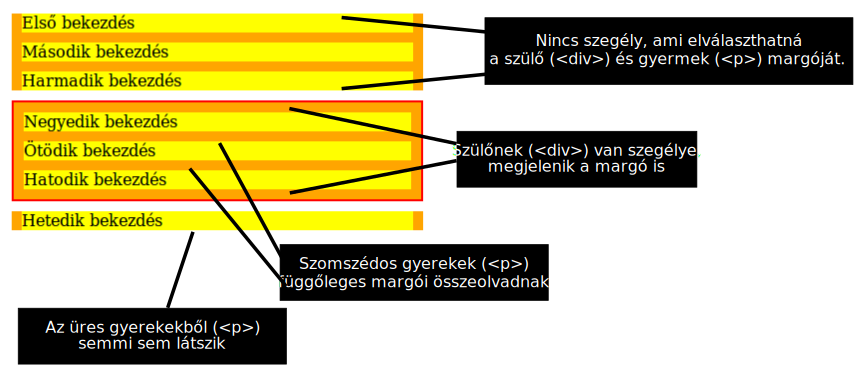
\includegraphics[scale=0.55]{margok.pdf}
  \end{center}
\end{frame}
